\section{Introduction}
\label{sec:intro}

\begin{figure}[t]
  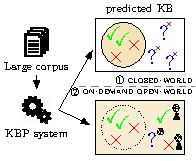
\includegraphics[width=\columnwidth]{figures/overview}
  \caption{\label{fig:task}
  In knowledge base population (KBP), systems construct a knowledge base (KB) containing \textit{facts} about \textit{entities} 
  %such as where a person was born or who a company's founder is, 
  from a large document corpus documents.
  \encircle{1}
  Under the closed-world evaluation methodology, only those facts that intersect with an existing set of annotated facts
  %, usually constructed from other output of other systems,
  are considered to be true and all others are assumed false.
  %This can significantly penalize a novel system that predicts new facts outside what has already been annotated.
  \encircle{2}
  In the on-demand open-world methodology, predicted facts that have never been annotated before are sampled and immediately evaluated through crowd-sourcing to provide an unbiased estimate of performance in an open-world setting.
  }
\end{figure}

% (1 page w/ figure)
% Goal: remind the reader what information extraction is, what its relation to knowledge base population is and why it is important. Hook question.
Harnessing the wealth of information present in unstructured text online has been and continues to be a long standing goal for the natural language processing community.
In particular, one approach to doing so has been to construct a \textit{knowledge base} storing information in a (possibly weak) relational schema, integrating the output of several information extraction tasks, including entity detection and linking, relation extraction and event extraction.
Knowledge bases such as YAGO, Freebase and Wikidata have shown immense value for question answering, search relevance, and potential in reasoning systems\needcite.

% TODO: This line would be nice to follow, but it's pending a cross-year evaluation.
% Significant effort and resources have been invested in improving the performance of knowledge base population (KBP) systems, but have our systems actually gotten better and if so, by how much?

% Goal: Setup analysis by describing TAC-KBP. Describe first problem and how we solve it.
The main way performance on the KBP task has been evaluated has been through the annual TAC-KBP competition organized by NIST.\@
% TODO: argue the merits of the TAC-KBP challenge and its evaluation.
The competition has invited more than \fake{300} submissions from at least \fake{40} different teams over the last 7 years (since 2009).
Each year, teams are provided a document corpus and a list of query entities, for example ``Carrie Fisher'', to find facts for.
The proposed facts from each participating team are \emph{pooled} together and evaluated by human annotators.
While scores of top performing teams have improved, they remain under \fake{35\% \fone}.
In contrast, human evaluators provided access to simple text search for \fake{about 10 minutes} per query are able to identify far more facts and score about \fake{70\% \fone}.

% Analysis: biased!
%A number of confounding factors affect performance, including the performance of other systems, making comparisons difficult.
This plateau should be alarming for any researcher; if we are to break through this ceiling, we need to understand better what is holding us back.
Accordingly, we begin with an statistical analysis of the KBP evaluation in \sectionref{analysis}.
\plg{wouldn't call this key finding - just 'we find';
I think your key result is that you were able to get this whole system to work
}
Our key finding is that the pooling evaluation that teams use during development
produces scores that are on average 2\% points lower than they should be,
and therefore, this methodology is actually biased against novel system improvements.

% PL: I merged this paragraph into the paragraph below
\plg{would be good to merge this paragraph with the one below - because it's about the bias,
and can be shortened to be somewhat like what's in the abstract - it shouldn't be hard to explain}
The source of this bias arises because
the evaluation data only contains assessments for a subset of every candidate fact in the corpus
and there is no good way to score a predicted fact that is not part of this subset.
In particular, the evaluation data consists only of the candidate facts
``pooled'' together from systems that participated during the original
competition and were subsequently assessed by human annotators.

% Describe pooling bias, connect to IR
This \emph{pooling bias} has been studied in the information retrieval community\needcite,
%which bears many similarities to the knowledge base population task,
%e.g.\ both tasks
which also seeks to find ``relevant'' information from a large document corpus that is infeasible to exhaustively annotate.
\plg{insert brief description of pooling bias}
However, assessing the quality of system outputs is relatively objective in the context of knowledge base population.
This enables us to employ non-expert crowdworkers to accurately judge novel output submitted by teams during development.
\plg{I'm not sure the 'objective, therefore crowdsourcing' is convincing -
'relevance' also lends itself to crowdsourcing, which is what is done in IR too;
need to find something else to contrast, or just say we borrow ideas from IR?
}

% Better statistics
Another, perhaps intangible, obstacle in developing better KBP systems is the slow feedback loop that researchers face in testing their developments: they must wait a year for the next TAC-KBP challenge followed by several months to receive their test scores.
We propose a new online evaluation protocol that automates the process of query selection to provide more precise estimates of instance-level and entity-level evaluation metrics than the current methodology.
The evaluation protocol uses a clever combination of annotation of pooled output, exhaustive annotation on a subset of documents and correlations between unassessed outputs to produce unbiased estimates of precision and recall.
\plg{I'd focus this paragraph on the better statistical properties because that's your technical
contribution; slow feedback should be moved to the next paragraph, which talks about the upshot
of what you've accomplished}

We simulate this evaluation protocol using the 2015 KBP corpus and find that we are able to confidently evaluate submissions within a budget of \fake{\$100/system} with a fixed cost of \fake{\$1000/corpus}.
The implementation of the online evaluation platform will be made available for submissions at \url{http://anonymo.us}.

\pl{would probably drop this or fold it in - seems to minor to standalone}
Of independent interest is a statistical analysis of submissions to past KBP challenges that allows us to make comparisons across years.

%The platform is easy to use and will have a fresh stream of documents.

%For these reasons, we propose and implement a new evaluation methodology: an online evaluation platform that teams can submit to as they develop their systems (\sectionref{design}).
%We use a combination of exhaustive, selective and estimative annotations to balance cost, accuracy and guaranteed unbiased estimates of precision, recall and $\fone$ scores at the mention and entity level.
% \pl{I don't see the 'online evaluation platform' as the immediate solution;
% what I'd expect is a more technical solution - how to do the crowdsourcing to deal
% with bias and reweighting to deal with variance;
% making it online seems to help with more community aspects,
% which can be argued as valuable, but that seems like a separate point}

%\cite{chaganty2016perspectives}

%Next, we measure the effect of the pooling methodology \pl{need to explain pooling in enough detail for people to appreciate the problem} and find that it is significantly biased against unpooled systems: when evaluating improvements to your KBP system, your scores on the evaluation data could be 4--7\% lower than they would be if you had submitted said system; if you are developing a new KBP system, the bias can be as much as 20\%.
%This is serious methodological problem that provides a barrier of entry for new teams and makes incremental improvements to systems a coin toss-- real improvements in results will easily pass unnoticed. 


% We find that there is a large amount of variance in the scores due to varying difficulties of the query entities which leads to wide confidence intervals on the reported results.
% We show that this variance can be reduced by standardizing scores across queries, a new metric that is able to discriminate between systems \todo{50\%} more effectively. 
% \pl{the variance doesn't seem to be the thing causing the plateau;
% certainly it doesn't explain the difference between 30\% and 80\%;
% seems the bias is more pressing and should be talked about first
% }


% TODO: We haven't tried doing a cross-evaluation yet -- this would basically mean we take a reference system and try and compare performance across years relative to this system.
% We use a method for score standarization (\refsec{analysis}) to compare scores across years and find that \todo{there is no statistically significant improvement in the last several years}.

